
\begin{figure}[H]
\centering
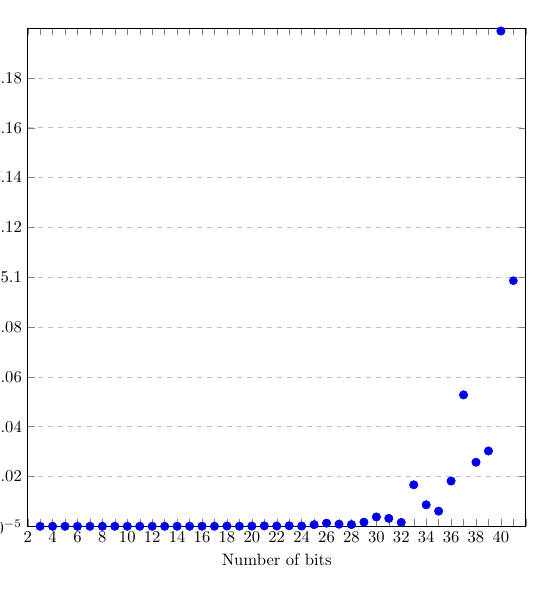
\begin{tikzpicture}[scale=0.6, trim axis left, trim axis right]
\begin{axis}[
    width=1\textwidth,
    height=1\textwidth,
    xlabel={Number of bits},
    ylabel={Time taken (s)},
    xmin=1.0, xmax=41,
    ymin=1.5e-05, ymax=10.2,
    xticklabels={2, , 4, , 6, , 8, , 10, , 12, , 14, , 16, , 18, , 20, , 22, , 24, , 26, , 28, , 30, , 32, , 34, , 36, , 38, , 40},
    xtick={1, 2, 3, 4, 5, 6, 7, 8, 9, 10, 11, 12, 13, 14, 15, 16, 17, 18, 19, 20, 21, 22, 23, 24, 25, 26, 27, 28, 29, 30, 31, 32, 33, 34, 35, 36, 37, 38, 39, 40, 41, 42, 43, 44, 45, 46, 47, 48, 49, 50, 51, 52, 53, 54, 55, 56, 57, 58, 59, 60, 61},
    ytick={0.0000150000000000000, 1.02001350000000, 2.04001200000000, 3.06001050000000, 4.08000900000000, 5.10000750000000, 6.12000600000000, 7.14000450000000, 8.16000300000000, 9.18000150000000},
    ymajorgrids=true,
    grid style=dashed,
]

\addplot+[
    blue,
    very thick,
    forget plot,
    only marks
    ]
    plot[
    very thick,
    error bars/.cd,
    y dir=plus,
    y explicit
    ]
    table[x=x,y=y,y error expr=\thisrow{y-max}] {
    x    y    y-max
    30	0.161975	0.0
37	1.311169	0.0
35	0.926861	0.0
32	0.849543	0.0
24	0.0333192	0.0002938
25	0.064159	0.0
26	0.043284	0.0
27	0.035551	0.0
20	0.0088994	0.0001436
21	0.005411	0.000181
22	0.0105919	0.0004511
23	0.0047538	6.42e-05
28	0.084783	0.0
29	0.191224	0.0
3	2.51e-05	8.19e-05
2	4.4e-05	0.000184
5	5.34e-05	7.86e-05
4	2.6e-05	3e-06
7	7.86e-05	7.94e-05
6	5.36e-05	7.84e-05
9	0.0001385	1.25e-05
8	0.0001217	7.63e-05
33	0.439183	0.0
39	10.141911	0.0
34	0.310229	0.0
38	1.542419	0.0
15	0.001766	2.1e-05
14	0.0009775	4.95e-05
11	0.0001041	7.39e-05
10	0.0003235	7.35e-05
13	0.0008575	6.35e-05
12	0.0001385	7.65e-05
17	0.0051386	5.84e-05
16	0.0011735	7.25e-05
19	0.0040232	0.0011198
18	0.0020383	0.0007457
36	2.69102	0.0
31	0.078828	0.0

    };

\addplot+[
    blue,
    very thick,
    forget plot,
    only marks
    ]
    plot[
    very thick,
    error bars/.cd,
    y dir=plus,
    y explicit
    ]
    table[x=x,y=y,y error expr=\thisrow{y-min}] {
    x    y    y-min
    30	0.161975	0.0
37	1.311169	0.0
35	0.926861	0.0
32	0.849543	0.0
24	0.0333192	-0.0001732
25	0.064159	0.0
26	0.043284	0.0
27	0.035551	0.0
20	0.0088994	-8.24e-05
21	0.005411	-4.2e-05
22	0.0105919	-0.0001079
23	0.0047538	-2.78e-05
28	0.084783	0.0
29	0.191224	0.0
40	5.029217	0.0
3	2.51e-05	-1.01e-05
2	4.4e-05	-2.4e-05
5	5.34e-05	-9.4e-06
4	2.6e-05	-1e-06
7	7.86e-05	-9.6e-06
6	5.36e-05	-9.6e-06
9	0.0001385	-2.5e-06
8	0.0001217	-1.07e-05
33	0.439183	0.0
39	10.141911	0.0
34	0.310229	0.0
38	1.542419	0.0
15	0.001766	-1.4e-05
14	0.0009775	-2.05e-05
11	0.0001041	-1.11e-05
10	0.0003235	-1.25e-05
13	0.0008575	-1.25e-05
12	0.0001385	-9.5e-06
17	0.0051386	-3.26e-05
16	0.0011735	-1.65e-05
19	0.0040232	-0.0001992
18	0.0020383	-0.0001203
36	2.69102	0.0
31	0.078828	0.0

    };

\end{axis}
\end{tikzpicture}
\vspace{-0.3cm}
\caption{Factors between 2 and 40 bits}\label{fig:PollardsRhoAlgorithmGrowingprimesbits240}
\end{figure}